% MIT 805 Big Data - Part 1 report skeleton
% Two-page main narrative + appendix. Compiles on Overleaf (pdfLaTeX).
%
% HOW TO USE THIS FILE
%   Every <<...>> is a placeholder. Fill it from output/report_numbers.json and
%   the CSVs the notebook writes. Delete the instructional comments as you go.
%   The 2-page limit applies to the main narrative only - push extra figures
%   past the \clearpage marker.

\documentclass[10pt,a4paper]{article}
\usepackage[margin=1.9cm]{geometry}
\usepackage{graphicx,booktabs,microtype,titlesec,hyperref,caption}
\usepackage[T1]{fontenc}
\hypersetup{colorlinks=true,urlcolor=blue!60!black,linkcolor=black}
\captionsetup{font=small,labelfont=bf,skip=3pt}
\titlespacing*{\section}{0pt}{1.4ex}{0.6ex}
\titlespacing*{\subsection}{0pt}{1.0ex}{0.4ex}
\titleformat{\section}{\normalfont\large\bfseries}{\thesection}{0.6em}{}
\setlength{\parskip}{0.35ex}
\pagestyle{empty}

\title{\vspace{-2.2em}\textbf{Large-Scale Analysis of NYC High Volume For-Hire
Vehicle Trip Records}\\[0.3em]
\large MIT 805 Big Data --- Part 1: Data Collection and Analysis}
\author{<<Name 1>> (<<student no.>>) \and <<Name 2>> (<<student no.>>)}
\date{\vspace{-1em}\small University of Pretoria \quad|\quad 3 September 2026}

\begin{document}
\maketitle
\vspace{-1.8em}

\noindent\textbf{Repository:} \url{https://github.com/<<user>>/<<repo>>}

% ---------------------------------------------------------------- 1 (2 marks)
\section{Dataset provenance, licence and suitability}

% Needed for full marks: reliable source, URL, licence/terms, academic suitability.
The dataset is the \emph{High Volume For-Hire Vehicle} (HVFHV) trip record
collection published by the New York City Taxi and Limousine Commission (TLC)
at \url{https://www.nyc.gov/site/tlc/about/tlc-trip-record-data.page}. It
records every trip dispatched by the four licensed high-volume operators ---
Uber (HV0003), Lyft (HV0005), Via (HV0004) and Juno (HV0002) --- and has been
published as a separate, more detailed series since February 2019. Files are
distributed as monthly Apache Parquet objects and mirrored in the AWS Open Data
Registry (\texttt{s3://nyc-tlc}).

The data is released under the NYC.gov Terms of Use as part of NYC Open Data,
which permits free public reuse, including academic research, with attribution
to the City of New York. It contains no rider, driver or vehicle identifiers,
and locations are generalised to 265 administrative taxi zones rather than GPS
coordinates, so no personally identifiable information is redistributed. The
TLC states that the records are submitted by the licensed bases and that it
makes no representation as to their accuracy --- a caveat we treat as an
analytical constraint in \S3 rather than a disqualifier.

% ---------------------------------------------------------------- 2 (3 marks)
\section{Scale and characteristics}

% Needed for full marks: raw, working AND processing sizes; format; records;
% variables; time period; relevant characteristics.
Table~\ref{tab:scale} reports the three required scales. Raw sizes were
established without downloading the archive by issuing an HTTP \texttt{HEAD}
request against each of the <<n>> published monthly files and summing
\texttt{Content-Length}.

\begin{table}[h]\centering\small
\caption{Dataset tiers. Parquet is columnar and compressed; the uncompressed
logical size is the volume Spark actually materialises.}
\label{tab:scale}
\begin{tabular}{@{}llrrr@{}}
\toprule
Tier & Period & Files & Parquet (GB) & Uncompressed (GB) \\
\midrule
Raw        & 2019-02 -- 2026-05 & <<n>>  & <<x>> & <<x>> \\
Working    & 2024-01 -- 2026-05 & <<n>>  & <<x>> & <<x>> \\
Processing & 2025-01 -- 2025-12 & 12     & <<x>> & <<x>> \\
\bottomrule
\end{tabular}
\end{table}

The processing tier holds <<N>> records across <<k>> columns. Each record is one
completed trip and carries four timestamps (request, on-scene, pickup,
dropoff), origin and destination zone identifiers, distance and duration,
seven itemised monetary fields, and five categorical service flags. We selected
calendar year 2025 because it is the first complete year under NYC congestion
pricing and the first carrying the \texttt{cbd\_congestion\_fee} column.

% ---------------------------------------------------------------- 3 (3 marks)
\section{Preparation and data quality}

% Needed for full marks: appropriate preparation PLUS meaningful discussion of
% missing data, duplicates, outliers, bias, representativeness.
\textbf{Schema evolution.} The series is not schema-stable. Files before 2021
omit \texttt{request\_datetime}, \texttt{trip\_miles}, \texttt{driver\_pay} and
the accessibility flags, and \texttt{cbd\_congestion\_fee} appears only from
2025. We therefore restricted the working tier to 2024 onward and read with
\texttt{mergeSchema} enabled.

\textbf{Missing data.} <<Summarise output/missingness.csv. Name the specific
columns and say why they are null rather than reporting a bare percentage ---
e.g. originating\_base\_num is absent for trips not routed through a distinct
originating base, and on\_scene\_datetime is unevenly populated across
operators, which biases any wait-time analysis toward operators that report
it.>>

\textbf{Validity.} We audited internal consistency rather than removing extreme
values by default (Table~\ref{tab:quality} / Appendix). <<Report counts for
zero-distance trips, non-positive durations, dropoff at or before pickup,
pickup before request, unknown zones 264/265, and implied speeds above
90\,mph.>> Cleaning retained <<x>>\% of records.

\textbf{Duplicates.} The schema carries no trip identifier, so duplicates can
only be defined on a composite key. <<x>>\% of records repeat on
(licensee, pickup, dropoff, PU, DO, fare, driver pay); these are plausibly
coincident genuine trips rather than errors, and we retain them.

\textbf{Representativeness.} The data covers only completed, matched trips in a
single city. Cancellations, unfilled requests and surge state are absent, so the
series measures \emph{served} demand, not demand.

% ---------------------------------------------------------------- 4 (4 marks)
\section{Exploratory data analysis}

% Needed for full marks: appropriate statistics/visualisations that IDENTIFY AND
% INTERPRET patterns. Do not just describe the charts - say what they mean.
<<2-3 paragraphs. Cover at minimum: market concentration between Uber and Lyft;
the weekly demand cycle (Fig.~\ref{fig:heat}) and what the Friday/Saturday late
-night ridge implies for fleet positioning; the wait-time profile and where it
degrades; shared-ride and WAV request-versus-match rates; the geographic
concentration of pickups; and the driver share of fares over the year.
Interpret each - a marker is looking for insight, not captions in prose form.>>

\begin{figure}[h]\centering
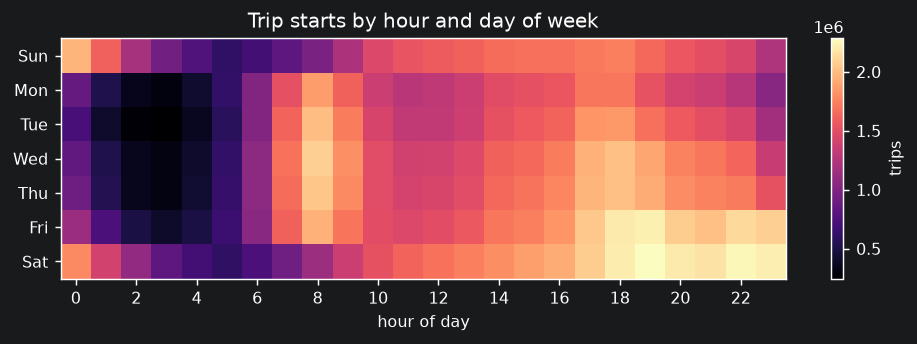
\includegraphics[width=0.92\linewidth]{../figures/fig4_hour_dow_heatmap.png}
\caption{Trip starts by hour of day and day of week, 2025.}
\label{fig:heat}
\end{figure}

% ---------------------------------------------------------------- 5 (4 marks)
\section{The seven Vs}

% Needed for full marks: applied to THIS dataset with EVIDENCE. Generic
% definitions score 1/4. Every V below must cite a number you computed.
\textbf{Volume.} <<x>> GB raw across <<n>> monthly files; <<N>> trips in the
processing year alone.

\textbf{Velocity.} A mean of <<x>> trips per day, roughly <<x>> per second
citywide. Crucially the \emph{generation} rate is real-time while the
\emph{publication} rate is monthly with a two-month lag --- so this is a
high-velocity process delivered as a batch product, which rules out the
operational use cases it superficially appears to support.

\textbf{Variety.} <<k>> columns spanning four timestamp types, categorical
licence codes, integer zone keys joined to an external CSV lookup and a
shapefile, decimal currency fields and Y/N flags; plus schema drift across
years.

\textbf{Value.} See \S6.

\textbf{Veracity.} <<Cite your validity-audit counts and the TLC's own accuracy
disclaimer.>>

\textbf{Variability.} <<Cite the COVID collapse visible in Fig.~A1, the seasonal
cycle, and the January 2025 introduction of cbd\_congestion\_fee.>>

\textbf{Volatility.} <<How long the data stays decision-relevant: TLC retains
records from 2009, but the two-month lag and post-congestion-pricing regime
change mean pre-2025 behavioural patterns have short operational shelf life.>>

% ---------------------------------------------------------------- 6 (2 marks)
\section{Value and limitations}

% Needed for full marks: clear value PLUS at least two meaningful limitations.
\textbf{Value.} <<Name stakeholders explicitly: TLC rulemaking on minimum driver
pay, where the observed driver share of fares is directly measurable;
congestion-pricing evaluation; accessibility equity, where the WAV
request-versus-match gap quantifies unmet demand from disabled passengers;
operator fleet positioning. Tie each to a number you computed.>>

\textbf{Limitations.} (i) \emph{Survivorship.} Only matched, completed trips are
recorded --- unfilled requests and cancellations are invisible, so the data
cannot measure latent demand or true service failure. (ii) \emph{No entity
identifiers.} Without driver, vehicle or rider keys, no retention, utilisation
or driver-earnings-per-shift analysis is possible; all inference is
trip-level. (iii) <<Optional third: zone-level granularity precludes
route-level analysis; single-city scope limits external validity.>>

\vspace{0.4em}
\noindent\rule{\linewidth}{0.4pt}
\clearpage % ---- appendix starts here; not counted in the 2-page narrative ----
\section*{Appendix}
% Supporting tables, figures and code output. Not counted in the 2-page limit.

\begin{table}[h]\centering\small
\caption{Validity audit on the processing tier.}\label{tab:quality}
\begin{tabular}{@{}lrr@{}}
\toprule
Check & Records & \% \\
\midrule
<<paste output/quality_checks.csv>> \\
\bottomrule
\end{tabular}
\end{table}

\begin{figure}[h]\centering
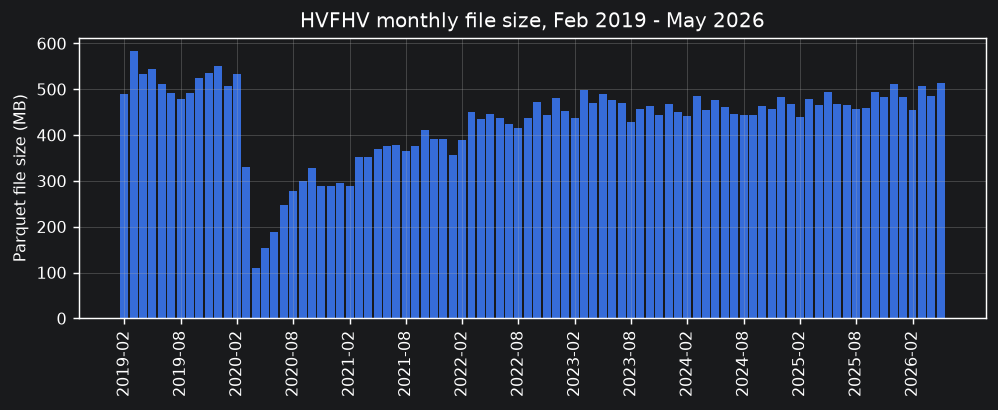
\includegraphics[width=0.95\linewidth]{../figures/fig_a1_monthly_file_size.png}
\caption{Monthly file size, Feb 2019 -- May 2026.}
\end{figure}

\begin{figure}[h]\centering
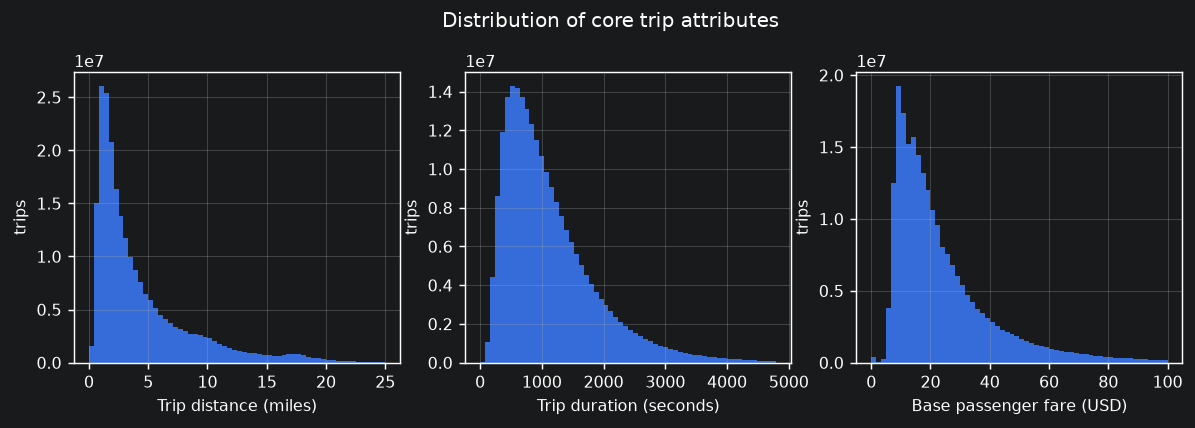
\includegraphics[width=0.95\linewidth]{../figures/fig2_distributions.png}
\caption{Distributions of distance, duration and fare.}
\end{figure}

\begin{figure}[h]\centering
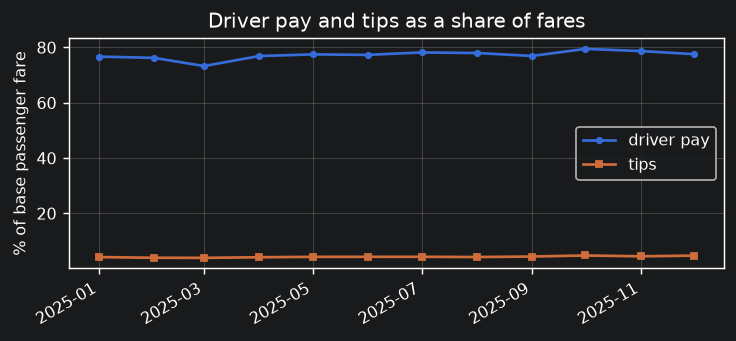
\includegraphics[width=0.8\linewidth]{../figures/fig7_driver_share.png}
\caption{Driver pay and tips as a share of base passenger fare.}
\end{figure}

\end{document}
